\chapter{Introduction}
\label{sec:introduction}

A number of problems can be addressed through optimization techniques.

\paragraph{Rocket.} Imagine you have to launch an ideal rocket with the goal of making it go as far as possible, and you have to choose the perfect angle. How do you choose it?

Optimization is about finding the best angle to maximize the distance the rocket touches the ground.

\simone{TODO: this section}


\section{Steps of Optimization Techniques}
\label{sec:introduction.steps}

Optimization can be defined as the selection of the most optimal element among all alternatives that satisfy certain criteria. In practice, it is sometimes computationally impractical to obtain the optimal solution. Consequently, a \textit{good} option is the one we settle for.

Optimization consists of four steps:
\begin{itemize}
    \item \textbf{Modeling}: in order to work on a problem with a computer, it is necessary to translate the problem into mathematical objects (variables, sets, functions, etc.) that represent it.
    
    \item \textbf{Solving}: Different problems have different characteristics and require analysis to determine the best technique. For example: 
    \begin{itemize}
        \item continuous/discrete: a deliveryman who has to decide how many pizzas to deliver each round must deliver an integer number of pizzas;
        \item linear/nonlinear;
        \item constrained/unconstrained: a car has a maximum speed;
        \item numerical/analytical. 
    \end{itemize}
    After the analysis of the characteristics, it is necessary to find the best algorithm for the solution of the problem.

    \item \textbf{Verification}: every algorithm always return a result (in a certain sense, even a segmentation fault is a result). But is it correct? At this stage, the result is evaluated to see if it makes sense.
    
    \item \textbf{Sensitivity analysis}: the algorithm may be perfect and return the correct result for the desired problem, but the problem may have been inappropriately modeled, e.g. some approximations are inevitable, but if you go too far you will get useless results in reality.
\end{itemize}

There are \underline{no global solutions}, but each problem is unique and requires different modeling, analysis, verification, and sensitivity analysis.

\section{Modeling}
\label{sec:introduction.modeling}

Mathematics can represent physical, economic, social, and other phenomenon. The process of creating a model is called modeling.

A good model must be:
\begin{itemize}
    \item \textbf{accurate enought}: a good model describes phenomena with a high degree of accuracy;
    \item \textbf{sufficiently simple}: a model that is too complex would require more sophisticated algorithms and many computing resources to solve;
    \item \textbf{sufficiently robust/wide}: a good model will be flexible enough to fit a wide range of scenarios.
\end{itemize}

The modeling process involves three steps:
\begin{enumerate}
    \item Identification of \textbf{state variables} (or decision variables): are things that can change in a problem (such as a robot's angle and a rocket's initial velocity). Decisione variables are represented as a column vector \( \mathbb{R}^n \) denoted by \( x \). For example, the variable of a car might be:
    \begin{align*}
        y &= \begin{bmatrix}
                \mathit{angle} \\
                \mathit{velocity} \\
                \mathit{distance} 
             \end{bmatrix}
    \end{align*} 

    \item Identification of a \textbf{ojective function} (or cost/gain function): is the function that evaluates how ``good'' a solution is. Formally it is a function \( f : \mathbb{R}^n \rightarrow \mathbb{R} \). In the car example, an objective function is the distance to the specified destination.
    
    \item Mathemarical description of the \textbf{constraints} (or circumstances): it specifies the constraints that the solution must have. For example, they can be given by physics (e.g. that the velocity must be positive). 
    Constraints take the form of real-valued functions in two possible forms:
    \begin{align*}
        h_i(x) = 0 && i = 1, ..., m && \mathrm{equality~constraints} \\
        g_j(x) \geq 0 && j = 1, ..., p && \mathrm{inequality~constraints}
    \end{align*}
    \simone{Capire bene cosa significa questa rappresentazione}

    The set of all solutions satisfying the constraints is called \textbf{feasible set} and is denoted as \( \Omega \).
\end{enumerate}

\begin{outline}
    \textbf{Example.} Consider a box in which we want to maximize the volume by fixing an area.

    \vspace{1em}
   
    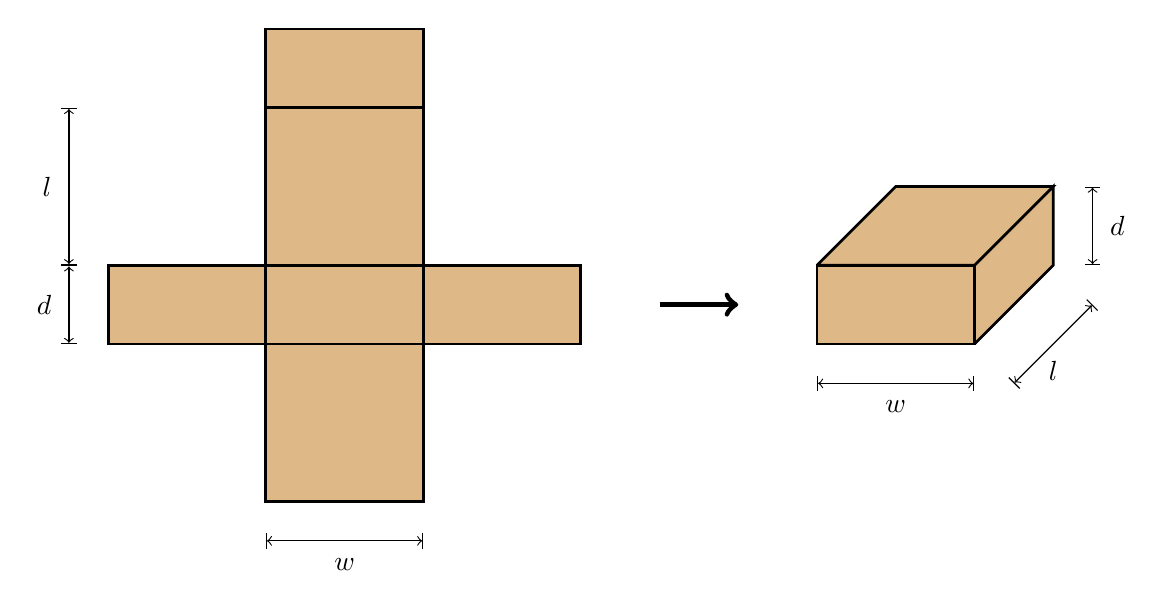
\begin{tikzpicture}
        \definecolor{boxcolor}{RGB}{222,184,135}
        
        % open box
        \draw[fill=boxcolor, line width=1pt] (3,1) rectangle (5,3);
        \draw[fill=boxcolor, line width=1pt] (3,3) rectangle (5,4);
        \draw[fill=boxcolor, line width=1pt] (3,3) rectangle (1,4);
        \draw[fill=boxcolor, line width=1pt] (5,3) rectangle (7,4);
        \draw[fill=boxcolor, line width=1pt] (3,4) rectangle (5,6);
        \draw[fill=boxcolor, line width=1pt] (3,6) rectangle (5,7);

        % quotes of open box
        \draw[|<->|] (0.5, 3) -- node[left=1mm]{\( d \)} (0.5, 4);
        \draw[|<->|] (0.5, 4) -- node[left=1mm]{\( l \)} (0.5, 6);
        \draw[|<->|] (3, 0.5) -- node[below=1mm]{\( w \)} (5, 0.5);

        % arrow
        \draw[->, line width=2px] (8, 3.5) -- (9, 3.5);

        % builded box
        \draw[fill=boxcolor, line width=1pt] (10,3) rectangle (12, 4);
        \draw[fill=boxcolor, line width=1pt] (12,3) -- (13, 4) -- (13, 5) -- (12, 4) -- (12, 3);
        \draw[fill=boxcolor, line width=1px] (10, 4) -- (12, 4) -- (13, 5) -- (11, 5) -- (10, 4);

        % quotes of closed box
        \draw[|<->|] (10, 2.5) -- node[below=1mm]{\( w \)} (12, 2.5);
        \draw[|<->|] (12.5, 2.5) -- node[below=1mm]{\( l \)} (13.5, 3.5);
        \draw[|<->|] (13.5, 4) -- node[right=1mm]{\( d \)} (13.5, 5);
   
    \end{tikzpicture}

    The problem can be modeled as follow:
    \begin{itemize}
        \item \textbf{Decision variables}: \( l, h, w \) in which \( l \) is the length, \( h \) is the height, and \( w \) is the width of the box.
        
        \item \textbf{Constraints}: \( 2lv + 2wh + 2lw = A \) constant. In other words, the area of the box has to be fixed and has to be the same in all the solutions.
        
        \item \textbf{Objective function}: \( V(l, h, w) = l \cdot h \cdot v \). Note: the goal is \( \underset{l, h, w}{\mathit{max}}~V(l, h, w) \).
    \end{itemize}

\end{outline}

\subsection{Formally}
\label{sec:introduction.modeling.formally}

The above definitions may give a good intuition of the concepts we will need throughout the course. However, it is necessary to define them formally.

\begin{definition}[feasible set]
    The feasible set, called \( \Omega \), is a set such that
    \[ 
        \Omega = \left\{ 
            x \in \mathbb{R}^n   
            \middle\vert
            \begin{array}{l}
                h_i(x) = 0, \quad i = 1, ..., m \\
                g_j(x) \geq 0, \quad j = 1, ..., p
            \end{array}
        \right\}
    \]
\end{definition}
\vspace{-1em}
It can be observed that \( \Omega \subseteq \mathbb{R}^n \).

\begin{definition}[objective function]
    A objective function is a function \( f \) such that \( f : \mathbb{R}^n \rightarrow \mathbb{R} \).
\end{definition}

\begin{definition}[minimization problem]
    Find the \( x \in \Omega \) that minimize \( f \).
\end{definition}

\begin{definition}[local minimum]
    A point \( x^* \in \Omega \) is a local minimum (or relative minimum) for \( f \) in \( \Omega \) if \( \exists \epsilon > 0 \) such that
    \[
        f(x^*) \leq f(x) \qquad \forall x \in \Omega \mathrm{~such~that~} \mathit{dist}(x, x^*) \leq \epsilon
    \]
\end{definition}

In other words, it is a point where the function has a lower value than all other nearby points.

\begin{tikzpicture}[scale=0.95]
    \draw (0,0) to[out=90,in=180] (2,2) to[out=0,in=180] (5,0) to[out=0,in=180] (7,3);
    \filldraw[black] (5,0) circle (2pt) node[anchor=north]{local min};
\end{tikzpicture}

\begin{definition}[strict local minimum]
    A point \( x^* \in \Omega \) is a strict local minimum for \( f \) in \( \Omega \) if \( \exists \epsilon > 0 \) such that
    \[
        f(x^*) < f(x) \qquad \forall x \in \Omega \mathrm{~such~that~} x^* \neq x \land \mathit{dist}(x, x^*) \leq \epsilon
    \]
\end{definition}

That is, the function has a higher (not equal) value at nearby points. In other words, "plateaus" are not allowed.

\begin{tikzpicture}[scale=0.95]
    \draw (0,0) to[out=90,in=180] (2,2) to[out=0,in=180] (5,0) to[out=0,in=180] (7,3);
    \filldraw[black] (5,0) circle (2pt) node[anchor=north]{strict local min};

    \draw (10,0) to[out=90,in=180] (12,2) to[out=0,in=180] (14,1.5) to[out=0,in=180] (15.5,1.5) to[out=0,in=-110] (16.5,2.5);
    \filldraw[black] (14.75,1.5) circle (2pt) node[anchor=north]{(non strict) local min};
\end{tikzpicture}

\begin{definition}[global minimum]
    A point \( x^* \in \Omega \) is a global minimum for \( f \) in \( \Omega \) if
    \[
        f(x^*) \leq f(x) \qquad \forall x \in \Omega
    \]
\end{definition}

In other words, the smallest local minimum.

\begin{tikzpicture}[scale=0.95]
    % \draw (0,1) to[out=-40,in=180] (3,2) to[out=0,in=180] (5,0) to[out=0,in=180] (7,3) to[out=0, in=190] (10, 2) to[out=10, in=-110] (11, 3);

    \draw 
        (0,2) to[out=-40, in=180] 
        (1,1) to[out=0, in=190] 
        (3,2) to[out=10, in=180]
        (5,0) to[out=0, in=210]
        (7, 2.5) to[out=20, in=180]
        (9,2) to[out=0, in=230]
        (10, 3)
        ;

    \filldraw[black] (5, 0) circle (2pt) node[anchor=north]{global min};
    \filldraw[black] (1, 1) circle (2pt) node[anchor=north]{local min};
    \filldraw[black] (9, 2) circle (2pt) node[anchor=north]{local min};
\end{tikzpicture}

In the case of a global minimum, we write \( f(x^*) = \underset{\Omega}{\mathtt{min}}f \) and \( x^* = \underset{\Omega}{\mathtt{argmin}} f \). 

Proceed in a similar manner to create the maximum (\( \mathtt{max} \)).